%------------------------
% CV in Latex
% Author : Sourabh Bajaj
% Modified by : Abhishek Ramanathapura Satyanarayana
% License : MIT
%------------------------

\documentclass[letterpaper, 10pt]{article}

\usepackage{latexsym}
\usepackage[empty]{fullpage}
\usepackage{titlesec}
\usepackage{marvosym}
\usepackage[usenames,dvipsnames]{color}
\usepackage{verbatim}
\usepackage{enumitem}
\usepackage[pdftex]{hyperref}
\usepackage{fancyhdr}
\usepackage{ragged2e}
\usepackage{comment}
\usepackage{graphicx,wrapfig}
\usepackage{fontawesome}
\graphicspath{{./images/}}

\pagestyle{plain}
\fancyhf{} % clear all header and footer fields
\fancyfoot{}
\cfoot{\thepage}
\renewcommand{\headrulewidth}{0pt}
\renewcommand{\footrulewidth}{0pt}

% Adjust margins
% \addtolength{\oddsidemargin}{-0.375in}
% \addtolength{\evensidemargin}{-0.375in}
% \addtolength{\textwidth}{1in}
% \addtolength{\topmargin}{-.5in}
% \addtolength{\textheight}{1.0in}
\usepackage[margin=0.6in]{geometry}

\urlstyle{same}
\raggedbottom
\raggedright
\setlength{\tabcolsep}{0in}

% Sections formatting
\titleformat{\section}{
    \vspace{-4pt}\scshape\raggedright\large
}{}{0em}{}[\color{black}\titlerule \vspace{-5pt}]

%-------------------------
% Custom commands
\newcommand{\resumeItem}[2]{
    \item\small{
        \textbf{#1}{: #2 \vspace{-2pt}}
    }
}

\newcommand{\resumeSubheading}[4]{
    \vspace{-1pt}\item
    \begin{tabular*}{0.97\textwidth}{l@{\extracolsep{\fill}}r}
        \textbf{#1} & #2 \\
        \textit{\small#3} & \textit{\small #4} \\
    \end{tabular*}\vspace{-5pt}
}

\newcommand{\resumeSubItem}[2]{\resumeItem{#1}{#2}\vspace{-4pt}}

\renewcommand{\labelitemii}{$\circ$}

\newcommand{\resumeSubHeadingListStart}{\begin{itemize}[leftmargin=*]}
\newcommand{\resumeSubHeadingListEnd}{\end{itemize}\vspace{-5pt}}
\newcommand{\resumeItemListStart}{\begin{itemize}}
\newcommand{\resumeItemListEnd}{\end{itemize}\vspace{-5pt}}

%-------------------------------------------
%%%%%%  CV STARTS HERE  %%%%%%%%%%%%%%%%%%%%%%%%%%%%
\pagenumbering{gobble}

\begin{document}

%--------IMAGE_AT_TOP_RIGHT--------
%\begin{comment}
    \begin{wrapfigure}[1]{r}{0.10\textwidth}
        \centering
        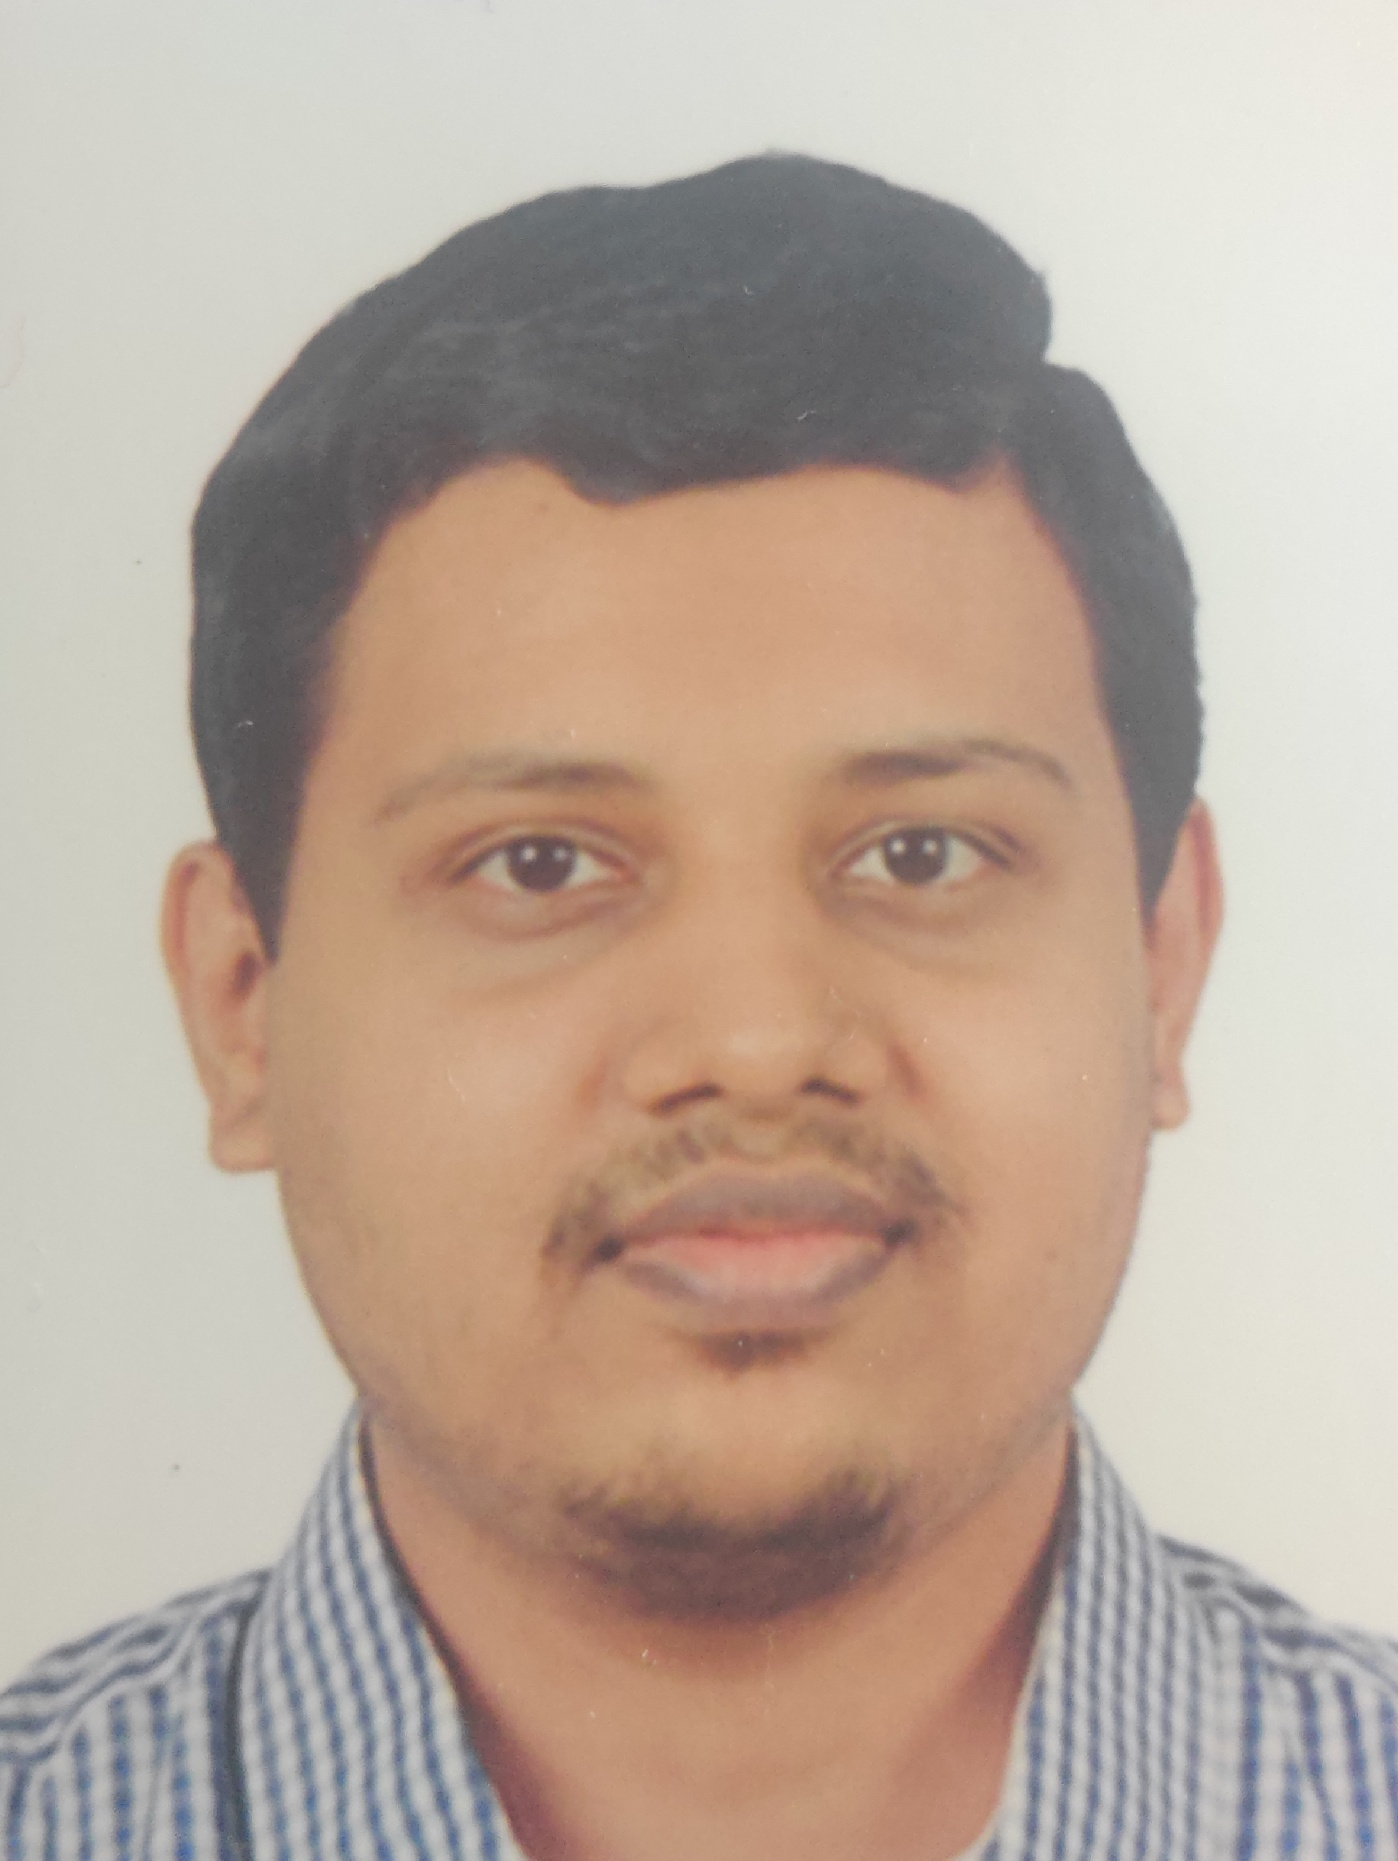
\includegraphics[width=1\linewidth]{images/abhishek_r_s.jpg}
    \end{wrapfigure}
    \paragraph{}
%\end{comment}

%----------HEADING-----------------
\begin{tabular*}{\textwidth}{l@{\extracolsep{\fill}}r}
    \textbf{{\Large ``Abhi"shek Ramanathapura Satyanarayana}}
    \\
    {(+31) 687353503, Groningen, The Netherlands (willing to relocate)}
    \vspace{0.15cm}
    \\
    
    \textbf{Email}: \href{mailto:abhishek.r.satyanarayana.4@gmail.com}{abhishek.r.satyanarayana.4@gmail.com} \hspace{0.1cm} 
    % \href{mailto:abhishekrsatyanarayana@gmail.com}{\faEnvelope} \hspace{0.1cm}
    \\
    \textbf{GitHub}: \href{https://github.com/AbhishekRS4/}{https://github.com/AbhishekRS4/} \hspace{0.1cm} 
    \textbf{HuggingFace}: \href{https://huggingface.co/abhishekrs4}{https://huggingface.co/abhishekrs4}
    \\
    \textbf{Personal Website}: \href{https://abhishekrs4.github.io/}{https://abhishekrs4.github.io/} \hspace{0.1cm} 
    \textbf{LinkedIn}: \href{https://linkedin.com/in/abhishek-r-s/}{https://linkedin.com/in/abhishek-r-s/} \hspace{0.1cm}
    %\href{https://drive.google.com/drive/folders/0Byk-dMy2pBxeX21IbmRlWFExNFk?usp=sharing}{\faFilesO}
    \\
    
\end{tabular*}

\section{About me}
I am a graduate Artificial Intelligence (AI) Engineer from the University of Groningen. I am a motivated, talented, hardworking, and fast-learning professional. I am interested in a role in the field of AI with a long-term goal of contributing towards improving the various aspects of human lives and the environment through continuous development and deployment of AI applications that can have a significant impact on the real world. In my free time, I usually do one of the following --- playing badminton with friends, playing chess, listening to music, watching technology videos, going for walks.

%-----------RESEARCH INTERESTS----------------- [old]
\begin{comment}
    \section{Research Interests}
        \resumeSubHeadingListStart
            \item{Artificial Intelligence, Machine Learning, Deep Learning, Computer Vision, Robot Perception}\\
        \resumeSubHeadingListEnd
\end{comment}


%-----------EDUCATION-----------------
\section{Education}
    \resumeSubHeadingListStart
        \resumeSubheading
            {M.Sc. in Artificial Intelligence}{Groningen, The Netherlands}
            %{\underline{\href{https://www.rug.nl/masters/artificial-intelligence/}{University of Groningen [RUG]}}}{Sep 2021 - present}
            {University of Groningen [RUG]}{Sep 2021 - Oct 2023}
            \resumeSubHeadingListStart
                \resumeItem{Thesis}{For my AI Master's thesis I worked on a research project titled \textbf{Enhancing depth estimation for Transparent objects}. In this research, we proposed a novel encoder-decoder architecture that outperformed the state-of-the-art method.}
                \resumeItem{Relevant Courses}{Machine Learning, Deep Learning, Pattern Recognition, Handwriting Recognition, Cognitive Robotics, Robotics for AI, Computer Vision, Natural Language Processing, Deep Reinforcement Learning, Intro to Data Science.}
                \resumeItem{Grade}{GPA: 8.3/10, Thesis: 8.5/10}
            \resumeSubHeadingListEnd

        \resumeSubheading
            {Honours Master's in High Tech Systems and Materials (HTSM)}{Groningen, The Netherlands}
            %{\underline{\href{https://www.rug.nl/education/honours-college/htsm-masterprogramme/}{Honours College, University of Groningen}}}{Nov 2021 - Jun 2023}
            {Honours College, University of Groningen}{Nov 2021 - Jun 2023}
            \resumeSubHeadingListStart
                \resumeItem{Masterwork}{For my HTSM Masterwork, I worked on a research project titled \textbf{Oil Spill Segmentation using Deep Encoder-Decoder models}. In this project, we developed and evaluated the performance of popular deep encoder-decoder models for the oil spill segmentation task. The best-performing model has also been deployed to HuggingFace.}
                \resumeItem{Grade}{GPA: 7.9/10, Masterwork: 9/10}
            \resumeSubHeadingListEnd
        
        \resumeSubheading
            {B.Tech. in Information Technology}{Surathkal, Mangaluru,  India}
            %{\underline{\href{https://www.nitk.ac.in/}{National Institute of Technology Karnataka [NITK]}}}{Jul 2012 - May 2016}
            {National Institute of Technology Karnataka [NITK]}{Jul 2012 - May 2016}
            \resumeSubHeadingListStart
                \resumeItem{Grade}{CGPA: 8.3/10}
            \resumeSubHeadingListEnd
    \resumeSubHeadingListEnd

%-----------EXPERIENCE-----------------
\section{Experience}
    \resumeSubHeadingListStart
        \resumeSubheading{Teaching Assistant (Part-time)}{Groningen, The Netherlands}{Faculty of Science and Engineering (FSE), University of Groningen}{May 2023 - Jun 2023}
            \resumeSubHeadingListStart
                \resumeItem{Responsibilities}{I worked as a TA for  \href{https://ocasys.rug.nl/current/catalog/course/WMAI019-05}{\textit{Handwriting Recognition}} course during which I monitored the weekly lab sessions, mentored some teams regarding their progress in the course project and graded the course projects.}
                \resumeItem{Skills}{Teamwork, Teaching, Time management, Communication, Python.}
            \resumeSubHeadingListEnd
        
        \resumeSubheading{Teaching Assistant (Part-time)}{Groningen, The Netherlands}{Faculty of Science and Engineering (FSE), University of Groningen}{Feb 2023 - Apr 2023}
            \resumeSubHeadingListStart
                \resumeItem{Responsibilities}{I worked as a TA for  \href{https://ocasys.rug.nl/current/catalog/course/WMAI017-05}{\textit{Deep Learning}} and \href{https://ocasys.rug.nl/current/catalog/course/WMCS015-05}{\textit{Computer Vision}} courses. I monitored the weekly lab sessions and graded assignments for both courses. I also invigilated the exam for the Deep Learning course.}
                \resumeItem{Skills}{Teamwork, Teaching, Time management, Communication, Python, Matlab.}
            \resumeSubHeadingListEnd
    
        \resumeSubheading{Teaching Assistant (Part-time)}{Groningen, The Netherlands}{Faculty of Science and Engineering (FSE), University of Groningen}{Sep 2022 - Nov 2022}
            \resumeSubHeadingListStart
                \resumeItem{Responsibilities}{I worked as a TA for  \href{https://www.rug.nl/ocasys/fwn/vak/show?code=WMAI003-05}{\textit{Cognitive Robotics}} and \href{https://www.rug.nl/ocasys/fwn/vak/show?code=WMCS002-05}{\textit{Introduction to Data Science}} courses during which I monitored the weekly lab sessions and graded assignments for both courses. I graded the course projects for the Cognitive Robotics course. For the Introduction to Data Science course, I invigilated the course exam, gave a presentation to the students on using Git and GitLab for course assignments, and maintained the GitLab assignment repositories for the teams.}
                \resumeItem{Skills}{Teamwork, Teaching, Time management, Leadership, Communication, Presentation, Python, Git, GitLab.}
            \resumeSubHeadingListEnd
    
        \resumeSubheading{Summer AI Intern}{IJmuiden, The Netherlands}{Tata Steel in Europe}{Jul 2022 - Aug 2022}
            \resumeSubHeadingListStart
                \resumeItem{Responsibilities}{I took part in this summer internship as a part of the \href{https://www.summerof.ai/}{Dutch Summer of AI}, edition 2022. I worked on supervised and unsupervised deep learning methods to classify and cluster images with steel surface defects. For the unsupervised task, I worked on a model as a proof of concept. For the supervised steel surface defect classification task, I worked on developing a production-ready AI model that achieved a $92\%$ accuracy. When deployed, this model would save at least $500$K Euros annually for Tata Steel. Our team won the award for \textbf{Solving the Most Valuable Problem}.}
                \resumeItem{Skills}{Teamwork, Time management, Communication, Presentation, Python, GitLab, Microsoft Azure, MLFlow.}
            \resumeSubHeadingListEnd

        \resumeSubheading{Teaching Assistant (Part-time)}{Groningen, The Netherlands}{University Medical Center Groningen (UMCG), University of Groningen}{Jun 2022 - Jul 2022}
            \resumeSubHeadingListStart
                \resumeItem{Responsibilities}{I worked as a TA for the Summer School Data Science and AI in Health. I was responsible for making sure that the assignment notebooks did not have any issues. I monitored and helped the students during the summer school.}
                \resumeItem{Skills}{Communication, Leadership, Time management, Python, Jupyter.}
            \resumeSubHeadingListEnd

        \resumeSubheading{Internship (Part-time)}{Drachten, The Netherlands}{Philips Consumer Lifestyle B.V.}{Nov 2021 - Jul 2022}
            \resumeSubHeadingListStart
                \resumeItem{Responsibilities}{For this internship, I worked as a part of an Honours Master's in HTSM. I was in a team in which we worked on a \textbf{report outlining different ways of developing a sustainable shaver by reducing the carbon footprint of one of the Philips shaver models}. We presented the top 5 ways of reducing the carbon footprint of the shaver. When some of our proposals are implemented, the carbon footprint of the shaver can be reduced by $16.6\%$ to $35\%$ depending on the choice.}
                \resumeItem{Skills}{Teamwork, Time management, Communication, Presentation.}
            \resumeSubHeadingListEnd

        \resumeSubheading{Research Associate (Machine Learning) in Autonomy}{Bengaluru, India}{Ati Motors}{Sep 2017 - Jun 2021}
            \resumeSubHeadingListStart
                \resumeItem{Responsibilities}{I worked mostly on research, prototyping, development, and deployment of Machine Learning, Deep Learning, Computer Vision, Robot Perception, and miscellaneous Algorithm solutions for autonomous cargo vehicles. In the learning algorithms, I worked mostly on object classification, object detection, and semantic segmentation in 2D images; and semantic segmentation in 3D LiDAR point cloud data. I also worked on benchmarking various ML models on multiple target hardware devices such as Nvidia's GPUs, Intel Movidius stick, and Nvidia Xavier embedded development board. I also worked on the development, deployment, and testing of LiDAR and camera sensor drivers, and raw and derived sensor data pipelines. I was also actively involved in support operations such as showcasing more than $15$ demos at potential customer sites and successful deployment activities at $3$ customer sites.}
                \resumeItem{Skills}{Communication, Teamwork, Time management, Leadership, Linux, Docker, Git, GitHub, Python, Jupyter, Streamlit, Flask, PyTorch, TensorFlow, TensorRT, Pandas, Scikit-learn, Scipy, OpenCV, C++, C.}
            \resumeSubHeadingListEnd

            % [old]
            % \resumeSubheading{Project Assistant Intern}{Bengaluru, India}{HPC Lab in SERC, Indian Institute of Science}{Jun 2016 - Dec 2016}
            % \resumeSubHeadingListStart
            %     \resumeItem{Responsibilities}{I worked on the implementation and benchmarking of data parallel algorithms on target GPU hardware.}
            %     \resumeItem{Skills}{C++, C.}
            % \resumeSubHeadingListEnd
            
            % \resumeSubheading{Technology Analyst Intern}{Mumbai, India}{Investment Banking, J P Morgan Chase}{May 2015 - Jul 2015}
            %     \resumeSubHeadingListStart
            %         \resumeItem{Responsibilities}{I worked on data analysis of real-time transaction data. I developed a dashboard application to filter out transactions and perform detailed analysis depending on the stakeholder requirements.}
            %         \resumeItem{Skills}{Communication, Teamwork, Time management, Leadership, Python, Data analysis, Jupyter, Pandas.}
            %     \resumeSubHeadingListEnd
    \resumeSubHeadingListEnd

\begin{comment}
%-----------PROFILES----------------- [old]
\section{Profiles}
    \resumeSubHeadingListStart
        \item{Linkedin: }
        \item{Github: \href{https://github.com/AbhishekRS4/}{\faGithub}}
            \item{Kaggle: \underline{\href{https://www.kaggle.com/abhishekrs4/}{https://www.kaggle.com/abhishekrs4/}}}
    \resumeSubHeadingListEnd
\end{comment}

%-----------PROJECTS----------------- [old]
\begin{comment}
\section{Projects}
    \resumeSubHeadingListStart
        \resumeSubItem{Developed a visualizer dashboard for analysis of data of Covid-19 infection in India}
        {This tool relies on data collected by an open-source project \href{https://www.covid19india.org/}{https://www.covid19india.org/}. The visualizer dashboard has multiple options to visualize Covid-19 infection data in India.}
        \resumeSubItem{Implementation of various Convolutional Neural Network models for Semantic Segmentation on Cityscapes and CamVid datasets}
        {Implemented various CNN models such as FCN, SegNet, UNet, LinkNet, PSPNet, DeepLab\_v3, Tiramisu on custom classes. The experiment is to study the various ideas proposed in research papers and its effects on performance of the model on validation set.}
        \resumeSubItem{Participated in TGS Salt Identification Challenge hosted on Kaggle}
        {Implemented custom CNN model using ideas from various research papers for salt segmentation in Kaggle competition. The model scored 0.811743 IoU on private test set. Our team finished in top 53\% of the leaderboard.}
        \resumeSubItem{Implementation of Convolutional Neural Network model based on Nvidia's research paper End to End Learning for Self-Driving Cars}
        {Implemented CNN model to predict steering angle from image on California Highway road dataset. The experiment is to reproduce the findings of the research paper that a CNN model can learn to predict steering angle from an image with reasonable performance.}
        \resumeSubItem{Classification of traffic sign images using German Traffic Sign Recognition Benchmark dataset}
        {Implemented CNN model for classification of traffic sign images on GTSRB dataset with 43 classes. The model scored 97.7\% accuracy on test set.}
        \resumeSubItem{Boston House Price Prediction}
        {Supervised Learning task of predicting the house median value for the Boston House dataset using various Regression techniques, Artificial Neural Network as part of mini project for Soft Computing Course. Tuning the hyper-parameters of ANN scored the best rmse among the various models.}
        \resumeSubItem{Comparison of Artificial Neural Network, Support Vector Regression (SVR), Genetic Algorithm-SVR}
        {Studied and experimented an IEEE paper which compares the three models ANN, SVR and GA-SVR using open source R and its packages as part of mini project for Data Warehousing and Data Mining Course. Tuning the hyper-parameters of ANN proved to be the best among the three models.}
        \resumeSubItem{Classification of handwritten digit images using MNIST dataset}
        {Implemented CNN model for classification of handwritten digit images on MNIST dataset with 10 classes. The model scored 99.47\% accuracy on test set.}
        \resumeSubItem{Denial of Service attack identification based on Reputation based Trust in Wireless Sensor Networks}
        {Identification of DoS attack based on Reputation based Trust in WSN using three different models RFSN model (a mathematical approach), human behavior model and ant colony optimization algorithm. This research was my Major Project (final year). We demonstrated that RFSN model could outperform other models in identification of the DoS attack.}
        \resumeSubItem{Data Parallel Algorithms}
        {Implementation of various Data Parallel Algorithms in OpenMP and CUDA C as part of Parallel Computing Course.}
        \resumeSubItem{Implementation of Machine Learning Algorithms}
        {Implemented various Machine learning algorithms in Python.}
    \resumeSubHeadingListEnd
\end{comment}

\section{Projects}
    \resumeSubHeadingListStart
        \resumeSubItem{Projects}
        {The projects can be found in my \href{https://github.com/AbhishekRS4/}{GitHub} and \href{https://huggingface.co/abhishekrs4}{HuggingFace} profiles.}
    \resumeSubHeadingListEnd

% --------SKILLS------------
\section{Skills}
    \resumeSubHeadingListStart
        \resumeSubItem{Soft Skills}
        {Teamwork, Time management, Communication, Leadership, Presentation, Teaching}
        \resumeSubItem{Programming languages}
        {Python, C++, C, Java, Matlab}
        \resumeSubItem{Version control (CI/CD)}
        {Git, GitHub, GitLab}
        \resumeSubItem{Frameworks}
        {Numpy, Scipy, Pandas, Matplotlib, Scikit, OpenCV, TensorFlow, PyTorch, Streamlit, Flask, FastAPI, etc.}
        \resumeSubItem{Miscellaneous Tech}
        {Linux, SQLite, MySQL, Docker, Kubernetes, MLFlow, HuggingFace, Microsoft Azure, AWS}
        \resumeSubItem{Languages}
        {English (professional), Dutch (elementary), Kannada (native), Hindi (professional)}
    \resumeSubHeadingListEnd

\begin{comment}
    % --------ONLINE COURSES------------
    \section{Self Learning Courses}
        \resumeSubHeadingListStart
            \item{Machine Learning, Coursera (Certification)}\\
            \item{Mathematics for Machine Learning Specialization, Coursera (Certification)}\\
            \item{Deep Learning Specialization, Coursera (Certification)}\\
            \item{Applied Data Science Specialization, Coursera (Certification)}\\
            \item{Python for Everybody Specialization, Coursera (Certification)}\\
            \item{Robotics - Perception, Coursera (Certification)}\\
            \item{An Intuitive Introduction to Probability, Coursera (Certification)}\\
            \item{Data Science Math Skills, Coursera (Certification)}\\
            \item{Fibonacci Numbers and Golden Ration, Coursera (Certification)}\\
            \item{Parallel Programming and Optimization for Intel Architectures, Colfax Research (Certification)}\\
        \resumeSubHeadingListEnd
\end{comment}


% --------AWARDS------------
\section{Notable Awards and Achievements}
    \resumeSubHeadingListStart
        \resumeSubheading{Student project award}{Groningen, The Netherlands}{University of Groningen}{2022-2023}
        \resumeSubHeadingListStart
            \resumeItem{GroNLP}{One of the best student project awards in the NLP course at the University of Groningen, for the word inflection relearning project.}
        \resumeSubHeadingListEnd

        \resumeSubheading{Most valuable problem award}{Amsterdam, The Netherlands}{Dutch Summer of AI, edition 2022}{2021-2022}
        \resumeSubHeadingListStart
            \resumeItem{Summer AI Intern at Tata Steel in Europe}{Our team won the award for Solving the Most Valuable Problem, among nine participating teams at the Dutch Summer of AI.}
        \resumeSubHeadingListEnd
    
        \resumeSubheading{Best solution award}{Groningen, The Netherlands}{Beta Business Days, edition 2022}{2021-2022}
        \resumeSubHeadingListStart
            \resumeItem{B \& S case study - Text recognition challenge}{Won the best solution award by developing a web application solution using the Azure cognitive services API.}
        \resumeSubHeadingListEnd
        
        \resumeSubheading{Student project award}{Groningen, The Netherlands}{University of Groningen}{2021-2022}
        \resumeSubHeadingListStart
            \resumeItem{Acute Myeloid Leukemia Prediction Challenge}{Our team won the $2^{nd}$ best performer award in the Acute Myeloid Leukemia Prediction Challenge conducted in the Introduction to Data Science course at the University of Groningen.}
        \resumeSubHeadingListEnd
    \resumeSubHeadingListEnd

% --------AWARDS------------ [old]
\begin{comment}
    \resumeSubheading{All India Engineering Entrance Examination [now replaced by JEE mains]}{India}{Secured a national rank of 6279 among 1200000 candidates}{2011-2012}
    \resumeSubheading{Karnataka Common Entrance Test [KCET] for Engineering}{India}{Secured a state rank of 404 among 80000 candidates}{2011-2012}
    \resumeSubheading{Pre-university Science quiz}{India}{3\textsuperscript{rd} prize in science quiz}{2011-2012}
    \resumeSubheading{Annual high school awards}{India}{3\textsuperscript{rd} best outgoing student award}{2009-2010}
    \resumeSubheading{Bharath ko jano (translation: Know about India)}{India}{2\textsuperscript{nd} prize in inter-high school quiz competition conducted by Bharath Vikas Parishad}{2009-2010}
    \resumeSubheading{Annual high school quiz competition}{India}{2\textsuperscript{nd} prize}{2009-2010}
    \resumeSubheading{Annual high school quiz competition}{India}{1\textsuperscript{st} prize}{2008-2009}
    \resumeSubheading{National Science Olympiad}{India}{1\textsuperscript{st} prize for my high school}{2007-2008}
    \resumeSubheading{Chess competitions in School}{India}{Various prizes in primary and high school including 3 first and 2 runner-up prizes}{2005-2010}
    \resumeSubheading{All India General Knowledge by Center for Human Resource Development}{India}{Completion of CHRD general knowledge competition with distinction}{2005-2006}
\end{comment}

\begin{comment}
    % --------EXTRA CURRICULAR ACTIVITY------------ [old]
    \section{Extra Curricular Activities}
        \resumeSubHeadingListStart
            \resumeSubheading{\underline{\href{https://www.imtex.in/}{IMTEX FORMING}} 2020 held at BIEC}{Bengaluru, India}{Represented Ati Motors}{Jan 2020}
            
            \resumeSubheading{Poster session held at Indian Institute of Science}{Bengaluru, India}{Represented Ati Motors}{Jul 2019}
            
            \resumeSubheading{\underline{\href{https://incident.nitk.ac.in/}{Incident-16}} (cultural festival of NITK)}{Surathkal, Mangaluru, India}{Team member that conducted the Gaming events of Incident-16}{Mar 2016}
            
            \resumeSubheading{TECHeshi’s castle at NITK IEEE tech festival}{Surathkal, Mangaluru, India}{Team member that conducted the event}{Dec 2012 - Jan 2013}
            
            %\resumeSubheading{Bengaluru district level science exhibition}{Bengaluru, India}{Presented on water conservation using rain water harvesting}{2007-2008}
            
            %\resumeSubheading{\underline{\href{https://www.janaagraha.org/bala-janaagraha/}{Bala Janagraha Civic learning programme}}}{Bengaluru, India}{Completed the civic learning programme in high school}{2007-2008}
        \resumeSubHeadingListEnd
\end{comment}


\begin{comment}
    % --------References------------ [old]
    \section{References}
        \resumeSubHeadingListStart
            \item
            {Dr. Geetha V \\
            Assistant Professor \\
            Department of Information Technology \\
            National Institute of Technology Karnataka, India \\
            Email: \underline{\href{mailto:geethav@nitk.edu.in}{geethav@nitk.edu.in}} \\
            Website: \underline{\href{https://infotech.nitk.ac.in/faculty/geetha-v}{https://infotech.nitk.ac.in/faculty/geetha-v}}}
            \item
            {Dr. Jaidhar C D \\
            Associate Professor \\
            Department of Information Technology \\
            National Institute of Technology Karnataka, India \\
            Email: \underline{\href{mailto:jaidharcd@nitk.edu.in}{jaidharcd@nitk.edu.in}} \\
            Website: \underline{\href{https://infotech.nitk.ac.in/faculty/jaidhar-c-d}{https://infotech.nitk.ac.in/faculty/jaidhar-c-d}}}
        \resumeSubHeadingListEnd
\end{comment}


%-------------------------------------------
\end{document}
